\documentclass[aspectratio=169, unicode, 10pt]{beamer}
\usepackage{fontspec}
\usepackage[]{zxjatype}
\usepackage[noto]{zxjafont}
\usepackage{color}
\XeTeXlinebreaklocale "ja"
\usefonttheme{professionalfonts}
%\usetheme{metropolis}
\usetheme{Goettingen}
\usecolortheme{orchid}
\title{研究室紹介}
\author{森田 太郎}
\institute[Sophia,NIMS]{Sophia University, National Institute for Materials Science}

\begin{document}
	\begin{frame}{}
		\titlepage
	\end{frame}

	\begin{frame}{目次}
		\tableofcontents[hideallsubsections]
	\end{frame}

	\section{研究テーマ}

	\begin{frame}
		\begin{block}{研究テーマ名}
			微量元素添加を行った内部スズ法Nb\textsubscript{3}Sn線材における拡散反応現象メカニズムの解明と超伝導特性向上の研究
		\end{block}
	\end{frame}


	\section{超伝導について}
	\begin{frame}{目次}
		\tableofcontents[currentsection, hideothersubsections]
		
	\end{frame}

	\subsection{超伝導とは}
	\begin{frame}{超伝導とは}
		\begin{columns}
			\begin{column}{0.5\linewidth}
				\begin{block}{超伝導の特徴}
					\begin{itemize}
						\item \textcolor{red}{電気抵抗がゼロ}
						\item 磁場が侵入しない
					\end{itemize}
				\end{block}
			\end{column}
			\begin{column}{0.5\linewidth}
				\begin{figure}
					\centering
					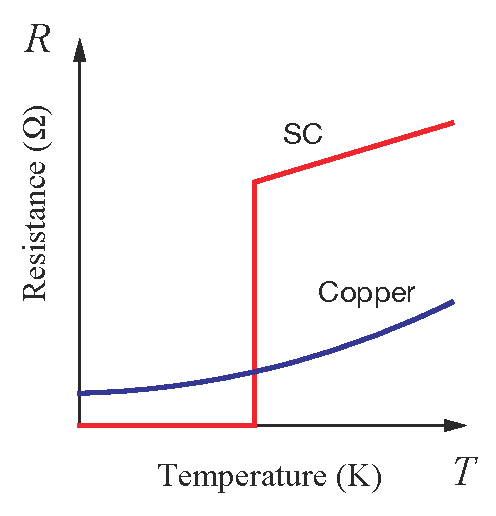
\includegraphics[width=0.95\linewidth]{figs/SC_temp.pdf}
				\end{figure}
			\end{column}
		\end{columns}
	\end{frame}

	\subsection{超伝導の領域(限界)}
	\begin{frame}{超伝導の領域}
		\begin{columns}
			\begin{column}{0.6\linewidth}
				\begin{block}{}
					\begin{itemize}
						\item ある一定の磁場,温度,電流で囲まれた領域で\textcolor{red}{超伝導}が発現する.
						\item 臨界値をそれぞれ\textcolor{red}{臨界磁場},\textcolor{red}{臨界温度},\textcolor{red}{臨界電流}と呼ぶ.
						\item 臨界温度,臨界磁場は材料によってほぼ決まっているが,臨界電流は\textcolor{red}{ピンニング特性を改善する}ことで特性が向上する.
					\end{itemize}
				\end{block}
			\end{column}
			\begin{column}{0.4\linewidth}
				\begin{figure}
					\centering
					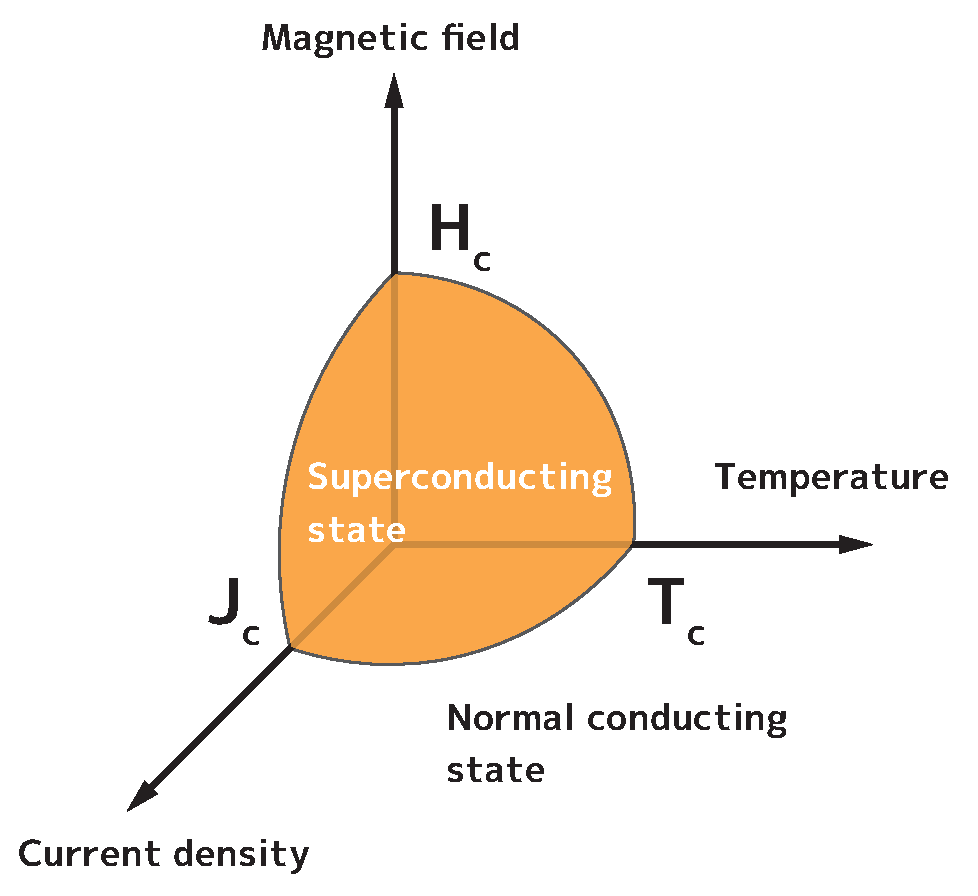
\includegraphics[width=\linewidth]{figs/SCstate.pdf}
				\end{figure}
			\end{column}
		\end{columns}
	\end{frame}

	\subsection{ピンニング機構とは}
	\begin{frame}{ピンニング機構について}
		\begin{columns}
			\begin{column}{0.5\linewidth}
				\begin{block}{}
					\begin{itemize}
						\item Type 2超伝導体内には磁束侵入.電流印可で磁束に\textcolor{red}{ローレンツ力}が働く.
						\item ローレンツ力により磁束が運動し始めると\textcolor{red}{起電力が発生し超伝導状態が破れる.}
						\item Type 2超伝導体内に侵入した磁束は\textcolor{red}{ピンニング点}と呼ばれる点で\textcolor{red}{ピン留め}される.
						\item \textcolor{red}{結晶粒界},不均質部などが主なピンニング点.
					\end{itemize}
				\end{block}
				
				\vspace{5mm}
				\centering
				\onslide<2>{\textcolor{red}{ピンニング点の密度を増加することで臨界電流が向上}}
			\end{column}
			\begin{column}{0.5\linewidth}
				\begin{figure}
					\centering
					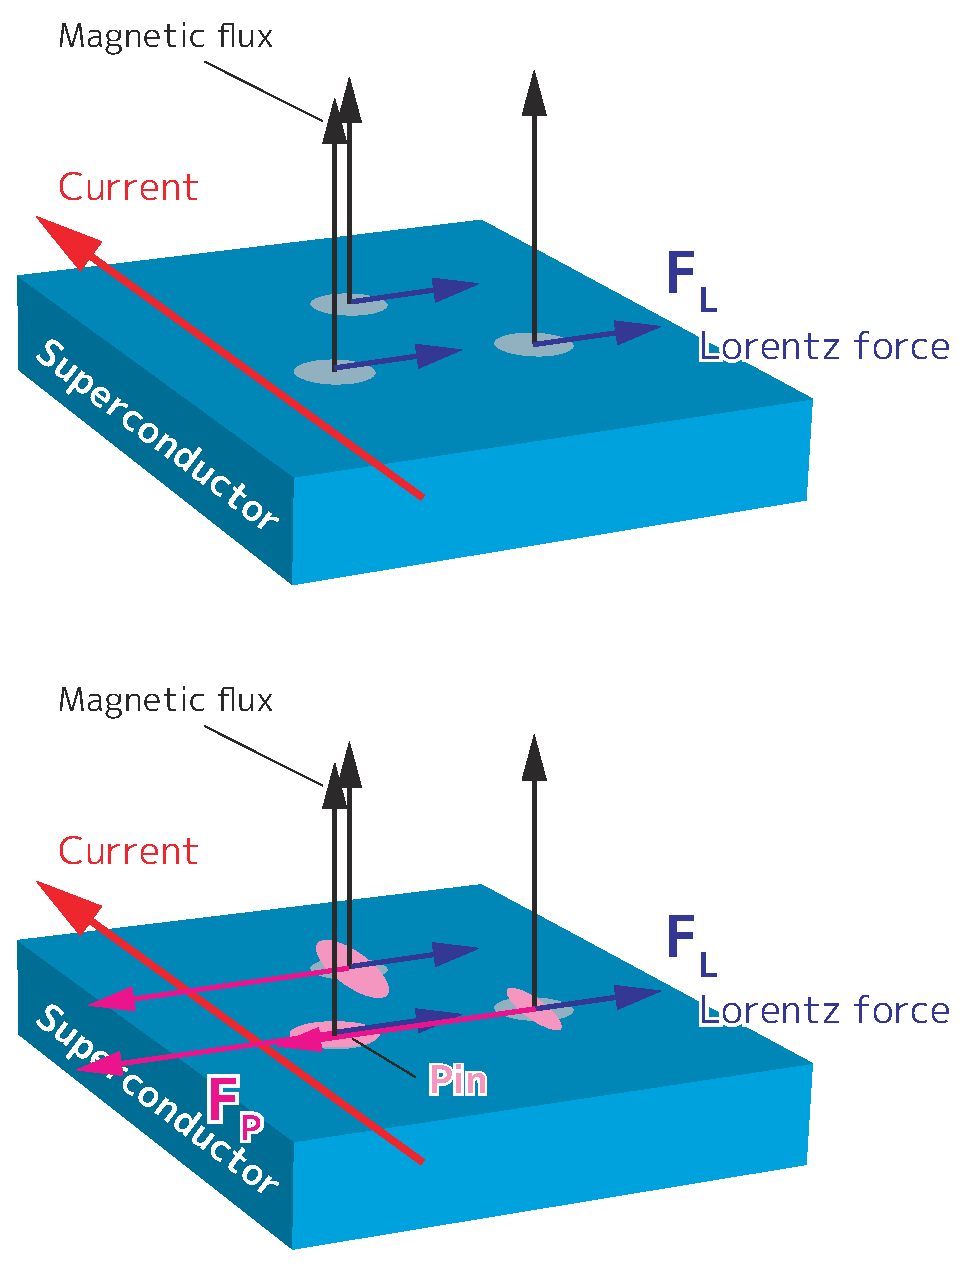
\includegraphics[width=0.8\linewidth]{figs/pinningforce.pdf}
				\end{figure}
			\end{column}
		\end{columns}
	\end{frame}

	\section{Nb\textsubscript{3}Snについて}
	\begin{frame}{目次}
		\tableofcontents[currentsection, hideothersubsections]
	\end{frame}

	\subsection{Nb\textsubscript{3}Sn線材の作り方}
	\begin{frame}{Nb\textsubscript{3}Sn線材の作り方}
		\begin{columns}
			\begin{column}{0.65\linewidth}
				\begin{enumerate}
					\item 前駆体となるパイプ.ロッドを用意・組み立て
					\item スエージング・冷間引抜加工\textcolor{red}{【伸線加工】}
					\item 1段階目熱処理 (for Sn/Cu mixing)
					\item 2段階目熱処理(for Nb\textsubscript{3}Sn formation)
				\end{enumerate}
			\end{column}
			\begin{column}{0.35\linewidth}
				\begin{figure}
					\centering
					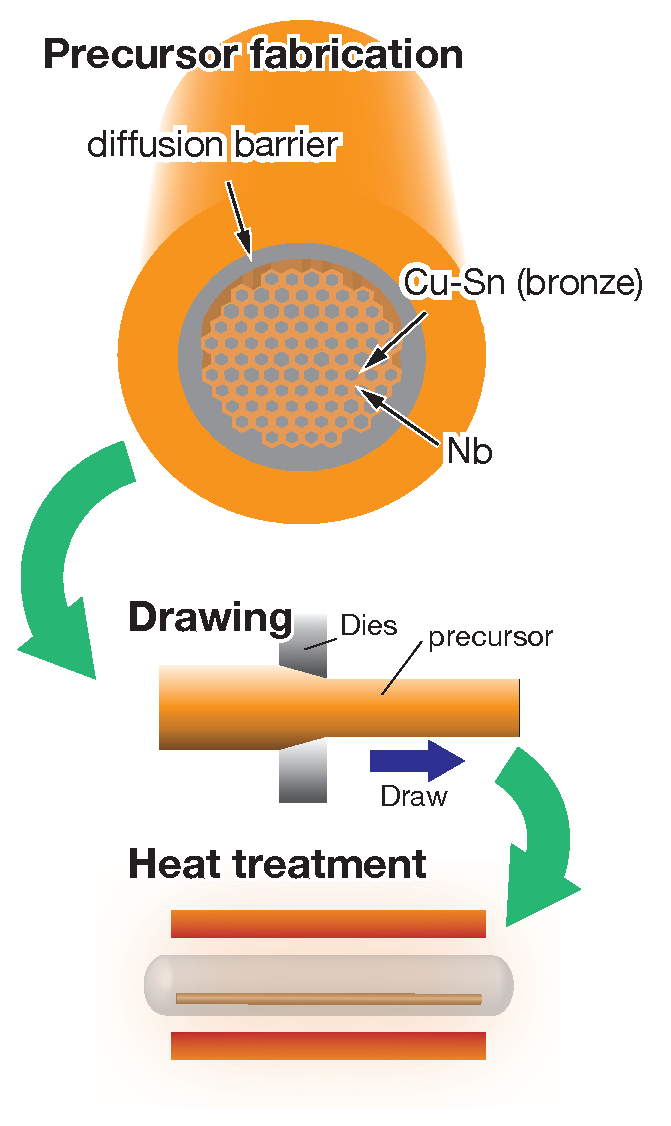
\includegraphics[width=0.9\linewidth]{figs/brozeProcessFabricationProcedure.pdf}
				\end{figure}	
			\end{column}
		\end{columns}
	\end{frame}

	\subsection{Nb\textsubscript{3}Snの特徴}
	\begin{frame}{Nb\textsubscript{3}Snについて}
		\begin{columns}
			\begin{column}{0.5\linewidth}
				\begin{block}{Nb\textsubscript{3}Snの特徴・メリット}
					\begin{itemize}
						\item 低温超伝導($T_\mathrm{c} = 18$~K).A15結晶組織.
						\item 工業化に適している.製造しやすく実績がある.
						\item 線材形状の柔軟性に富む.
						\item 優れた高磁界特性
					\end{itemize}
				\end{block}
				\vspace{5mm}
				\onslide<2>{次世代核融合炉や粒子加速器用マグネット材料として期待されている}
			\end{column}
			\begin{column}{0.5\linewidth}
				\begin{figure}
					\centering
					\includegraphics[width=0.3\linewidth]{figs/A15Structure.pdf}
				\end{figure}
				\begin{figure}
					\centering	
					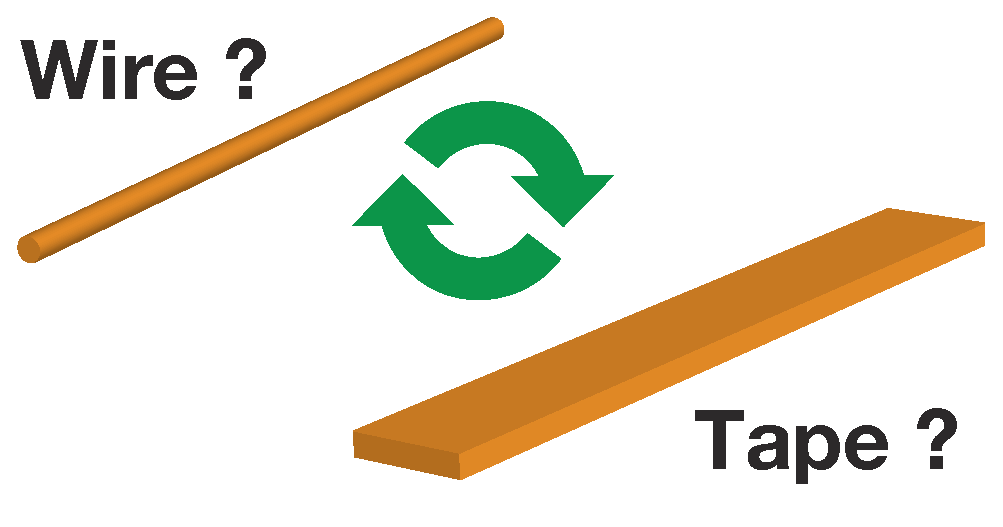
\includegraphics[width=0.85\linewidth]{figs/wireortape.pdf}
				\end{figure}
			\end{column}
		\end{columns}
	\end{frame}

	\subsection{Nb\textsubscript{3}Sn線材の課題}
	\begin{frame}{Nb\textsubscript{3}Sn線材の課題}
		\begin{block}{Nb\textsubscript{3}Snの課題点}
			\begin{itemize}
				\item \textcolor{red}{機械的な強度が著しく低い}
				\item 特性が飽和状態
			\end{itemize}
			\vspace{5mm}
			\pause{\textcolor{red}{次世代高磁場機器では\\
			高い$J_\mathrm{c}$特性,機械的強度が求められているため抜本的な解決策が必要}}
		\end{block}
	\end{frame}

	\subsection{Nb\textsubscript{3}Sn特性のキーポイント}
	\begin{frame}{Nb\textsubscript{3}Sn特性のキーポイント}
			\begin{block}{Nb\textsubscript{3}Sn層厚}
				\begin{itemize}
					\item Nb\textsubscript{3}SnはNbとSn間の\textcolor{red}{固相拡散反応}によって生成される
					\item 未反応Nbが最小,全体がNb\textsubscript{3}Snとなるとよい
				\end{itemize}
			\end{block}
			\begin{block}{Nb\textsubscript{3}Sn結晶粒径}
				\begin{itemize}
					\item 結晶粒径が小さいほど\textcolor{red}{結晶粒界は多くなる}
					\item 結晶粒界はピンニング点となる
				\end{itemize}
			\end{block}
			\begin{block}{Nb\textsubscript{3}Snの化学量論性}
				\begin{itemize}
					\item 化学式通りの組成を\textcolor{red}{化学量論性(Stoichiometry)という}
					\item Nb\textsubscript{3}Snは固相拡散反応によって生成されるので一般的にはNb\textsubscript{3}Sn層に組成勾配がある.できるだけNb:Sn = 3:1に近づける
				\end{itemize}
			\end{block}
	\end{frame}

	\subsection{従来のアプローチ}
	\begin{frame}{従来のアプローチ}
		\begin{columns}
			\begin{column}{0.6\linewidth}
				\begin{itemize}
					\item 従来線材は\textcolor{red}{Sn拡散長(Nbフィラメント径)},\textcolor{red}{仕込みNb:Sn:Cu比},\textcolor{red}{熱処理条件}を最適化することで特性の向上
					\item 上記最適化の研究はここ20年のうちに殆どやり尽くされている
				\end{itemize}	
				\vspace{5mm}
				\centering
				\onslide<2>{\Large \textcolor{red}{抜本的な解決策が必要}}
			\end{column}	
			\begin{column}{0.4\linewidth}
				\begin{figure}
					\centering
					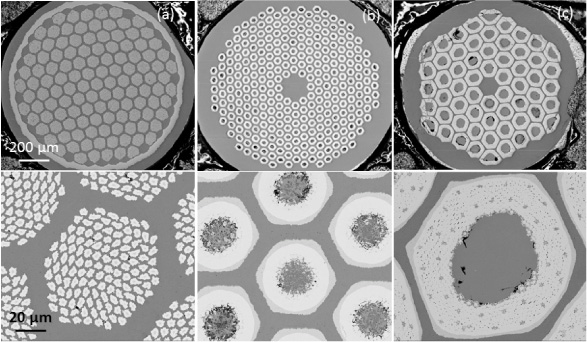
\includegraphics[width=\linewidth]{figs/rrpwire.png}
				\end{figure}
				\begin{figure}
					\centering
					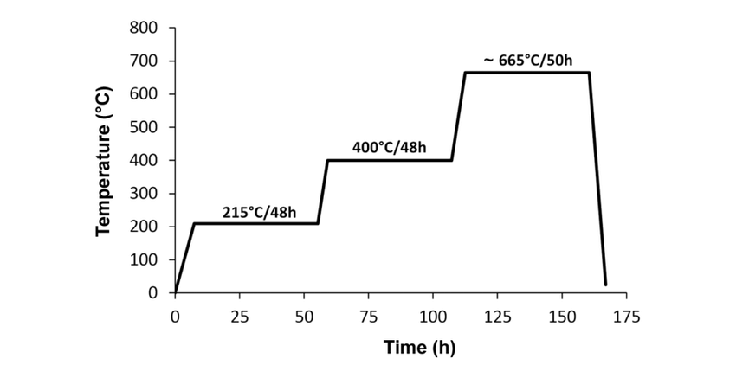
\includegraphics[width=\linewidth]{figs/rrpheattreatment.png}
				\end{figure}
			\end{column}
		\end{columns}
	\end{frame}

	\subsection{最近の動向}
	\begin{frame}{近年の世界動向}
		\begin{columns}
			\begin{column}{0.65\linewidth}
				\begin{itemize}
					\item 近年,\textcolor{red}{微細組織制御による特性向上}の研究が精力的に行われている
					\item Nb芯へのZr添加,Nb芯へのTa,Hf同時添加 → \textcolor{red}{結晶粒微細化}
					\item Nb-Ta-Hf線材のLayer $J_\mathrm{c}$がFCC要求性能を超えた
				\end{itemize}
			\end{column}
			\begin{column}{0.35\linewidth}
				\begin{figure}
					\centering
					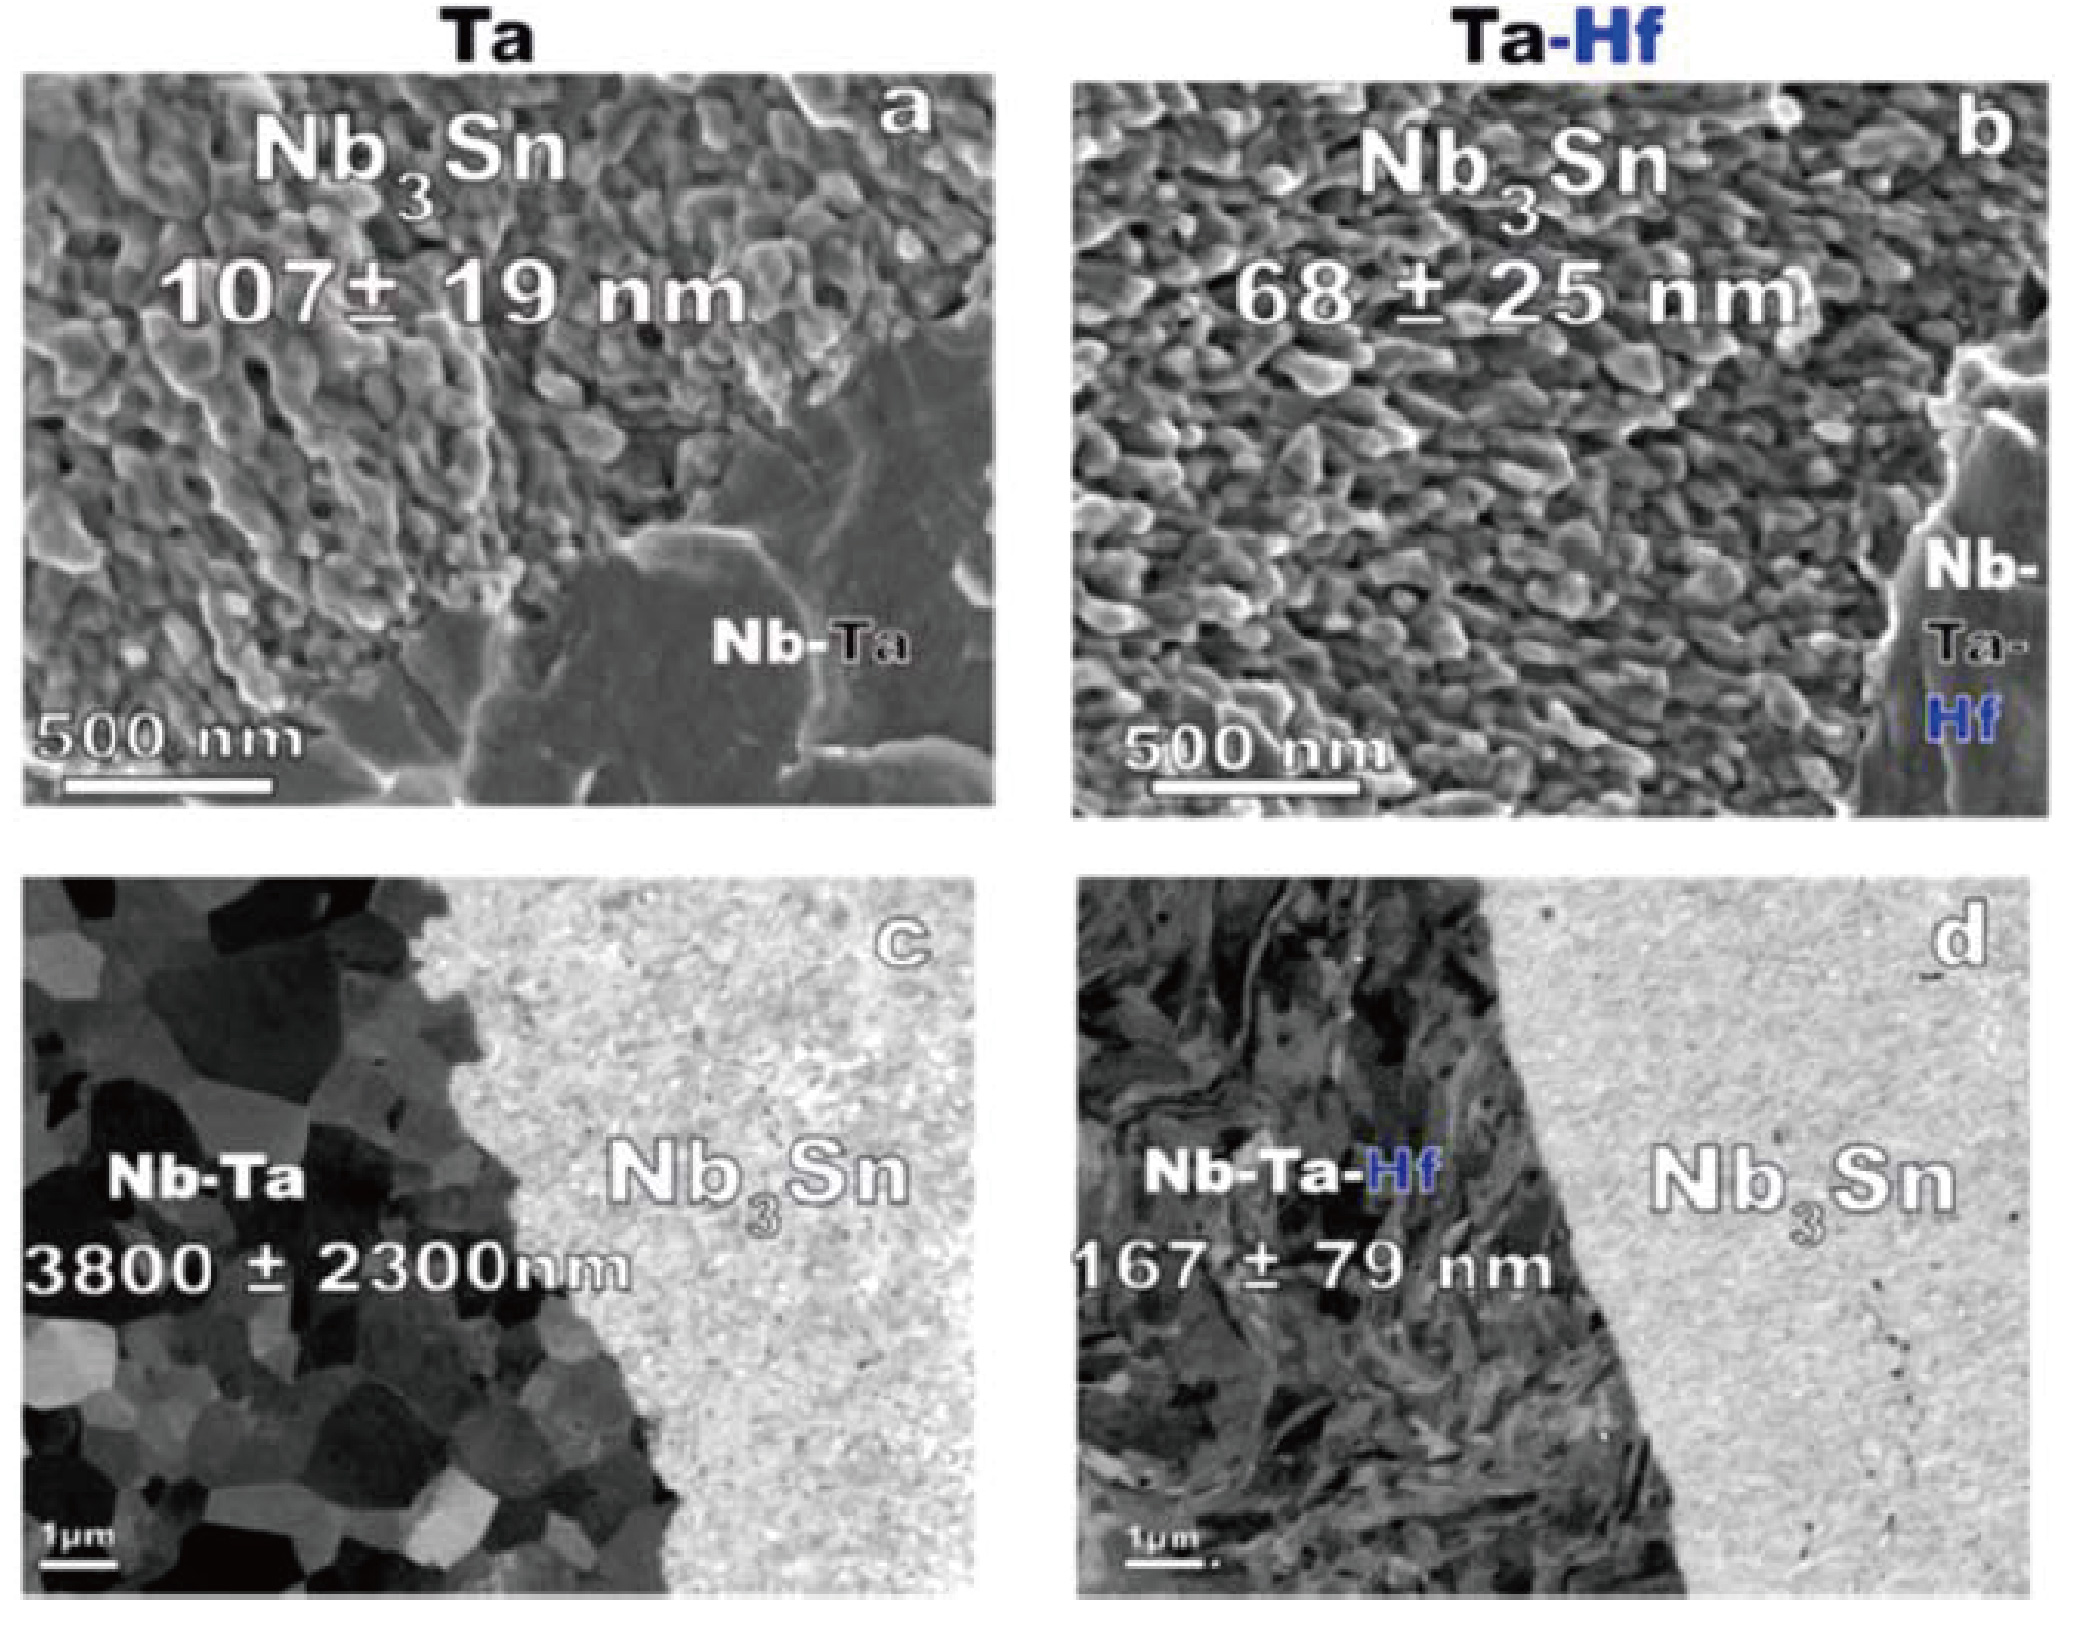
\includegraphics[width=\linewidth]{figs/NbTaHf.jpg}
				\end{figure}
			\end{column}
		\end{columns}

		\vspace{20pt}
		\pause{\large 微細組織には未だ特性向上のために\textcolor{red}{大きなポテンシャル}がある}
	\end{frame}

	\section{本研究について}
	\begin{frame}{目次}
		\tableofcontents[currentsection, hideothersubsections]
	\end{frame}

	\subsection{本研究の概要}
	\begin{frame}{本研究の概要}
		\begin{columns}
			\begin{column}{0.6\linewidth}
				\begin{itemize}
					\item 内部スズ法Nb\textsubscript{3}Sn線材におけるCu母材に元素添加
					\item 元素添加による\textcolor{red}{微細組織制御 → $J_\mathrm{c}$特性向上}
				\end{itemize}
				\begin{block}{Cu母材へのZn添加}
					\begin{itemize}
						\item Nb\textsubscript{3}Sn層生成促進(Sn拡散促進)
					\end{itemize}
				\end{block}
			\end{column}
			\begin{column}{0.4\linewidth}
				\begin{figure}
					\centering
					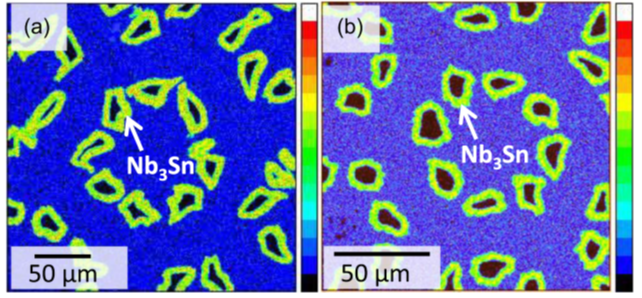
\includegraphics[width=\linewidth]{figs/effectofZnadditionNb3Snwidth.png}
				\end{figure}
			\end{column}
		\end{columns}

		\vspace{20pt}
		\centering
		\pause{Cu母材へのZn添加をベースに新たな元素を添加し微細組織制御を試みる}
	\end{frame}

	\subsection{研究方法・手順}
	\begin{frame}{研究方法・手順}
		\begin{enumerate}
			\item \textbf{前駆体作製} \\
				前駆体となるパイプ・ロッドを用意・組み立て
			\item \textbf{伸線加工} \\
				スエージング加工 → 冷間引抜加工
			\item \textbf{熱処理} \\
				はじめにSn拡散のための熱処理(550$^\circ$C程度),最後にNb\textsubscript{3}Sn生成のための熱処理(700$^\circ$C程度)
			\item \textbf{微細組織観察} \\
				FE-SEMによる微細組織観察,EDXによる元素分布観察,EBSDによる結晶構造,粒径分析
			\item \textbf{$I_\mathrm{c}$測定} \\
				10 $\sim$ 18~Tの外部印可磁場下で臨界電流$I_\mathrm{c}$を測定し,$J_\mathrm{c}$-$B$特性評価
		\end{enumerate}
	\end{frame}

	\subsection{研究結果}
	\begin{frame}{研究内容と結果}
		\centering
		{\LARGE Cu母材へのZn,Geの同時添加}
	\end{frame}

	\subsection{試料について}
	\begin{frame}{試料について}
		\begin{columns}
			\begin{column}{0.6\linewidth}
				\begin{block}{試料について}
					\begin{itemize}
							\item 母材:Cu-14wt\%Zn-1wt\%Ge合金
							\item Nb芯: pure Nb芯
							\item Sn芯: Sn-1.6wt\%Ti合金
							\item 伸線加工後,550$^\circ$C/100~hで熱処理 → 700 $\sim$ 750$^\circ$C/100~hで最終熱処理
					\end{itemize}
				\end{block}
				SEM,EDX分析,$I_\mathrm{c}$測定
			\end{column}
			\begin{column}{0.4\linewidth}
				\begin{figure}
					\centering
					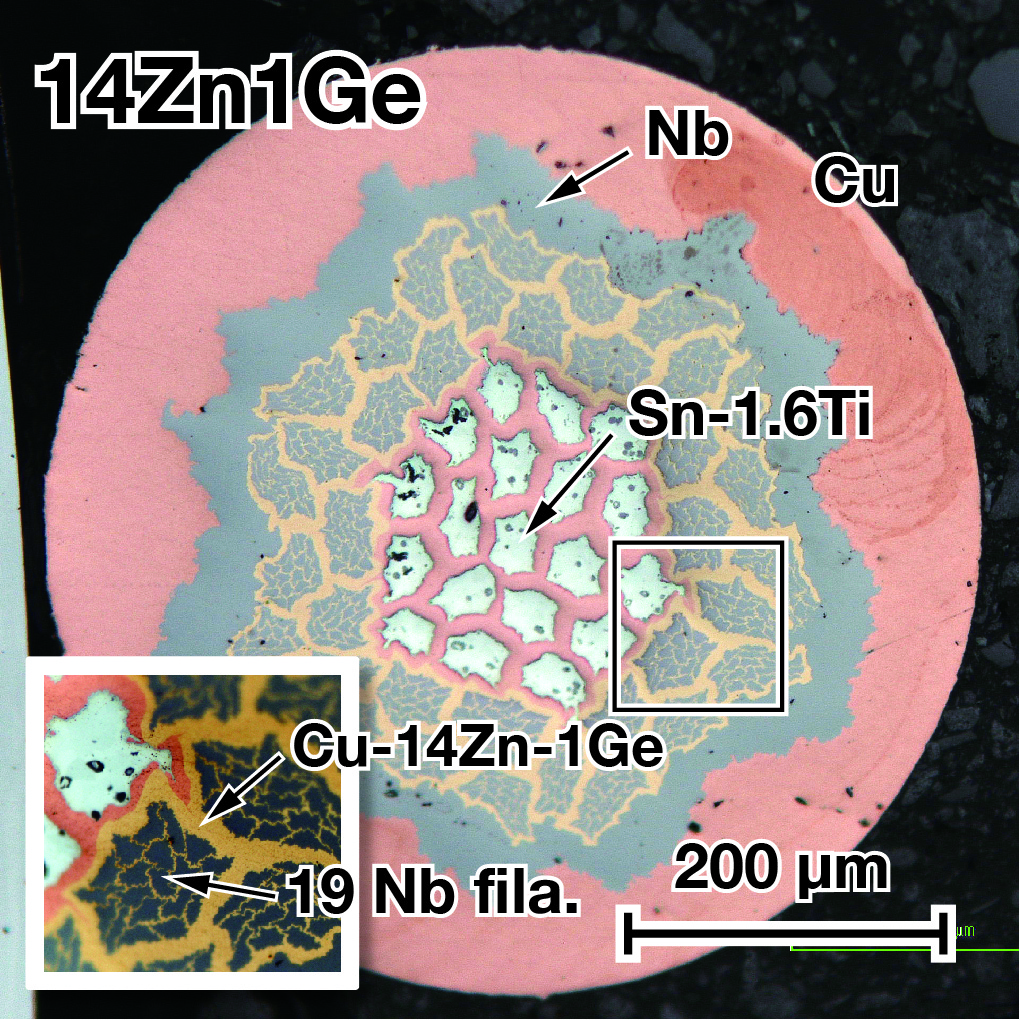
\includegraphics[width=\linewidth]{figs/14Zn1Ge_crossSection.jpg}
				\end{figure}
			\end{column}
		\end{columns}
	\end{frame}

	\subsection{元素分布}
	\begin{frame}{元素分布(EDX分析)}
		\begin{columns}
			\begin{column}{0.5\linewidth}
				\begin{itemize}
					\item Sn分布は不均一,未反応Nbあり
					\item Ti分布も不均一
					\item GeはNb\textsubscript{3}Sn層に分布
					\item ZnはNb\textsubscript{3}Snに固溶しない
				\end{itemize}
			\end{column}
			\begin{column}{0.5\linewidth}
				\centering
				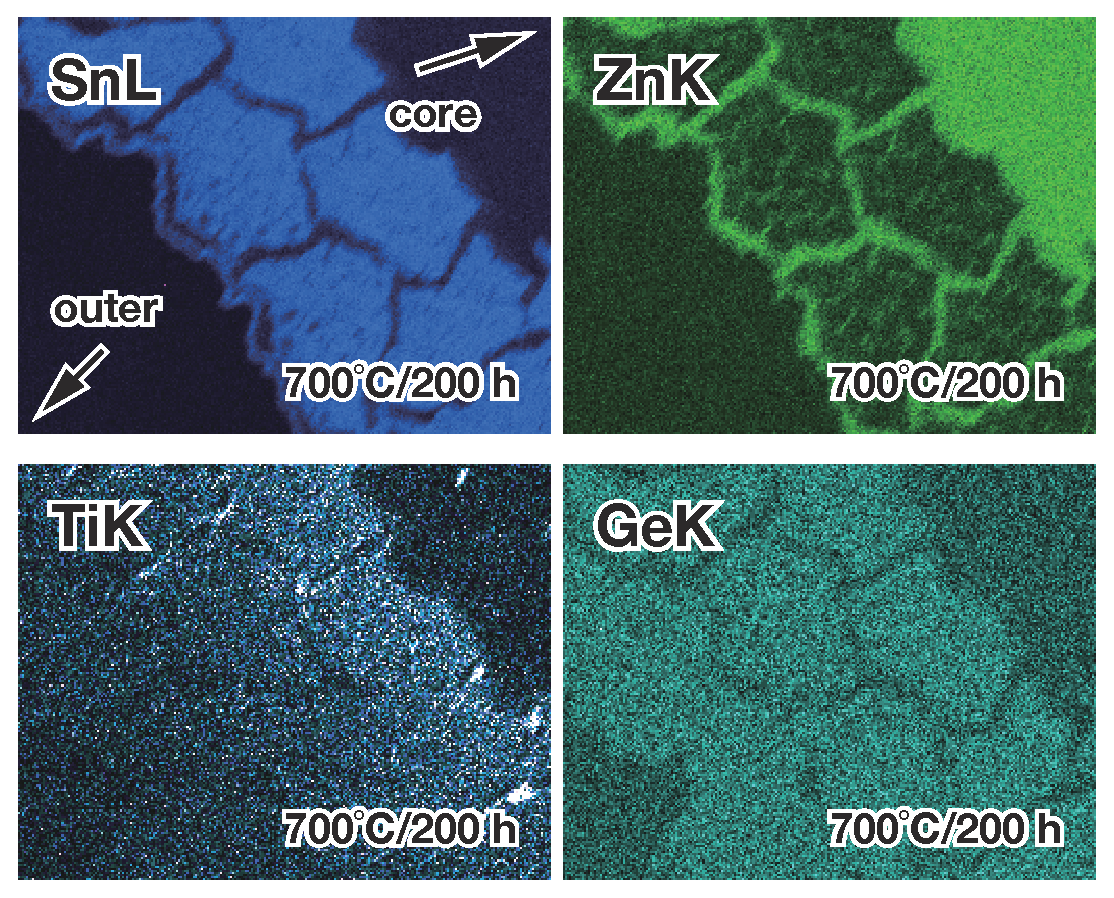
\includegraphics[width=\linewidth]{figs/14Zn1Ge-EDX.pdf}
			\end{column}
		\end{columns}
	\end{frame}

	\subsection{結晶組織観察}
	\begin{frame}{結晶組織(破断面・SEM像)}
		\begin{block}{800$^\circ$C $\times$ 50~h 熱処理}
			\begin{columns}
				\begin{column}{0.5\linewidth}
					\centering
					Ge添加無し\\
					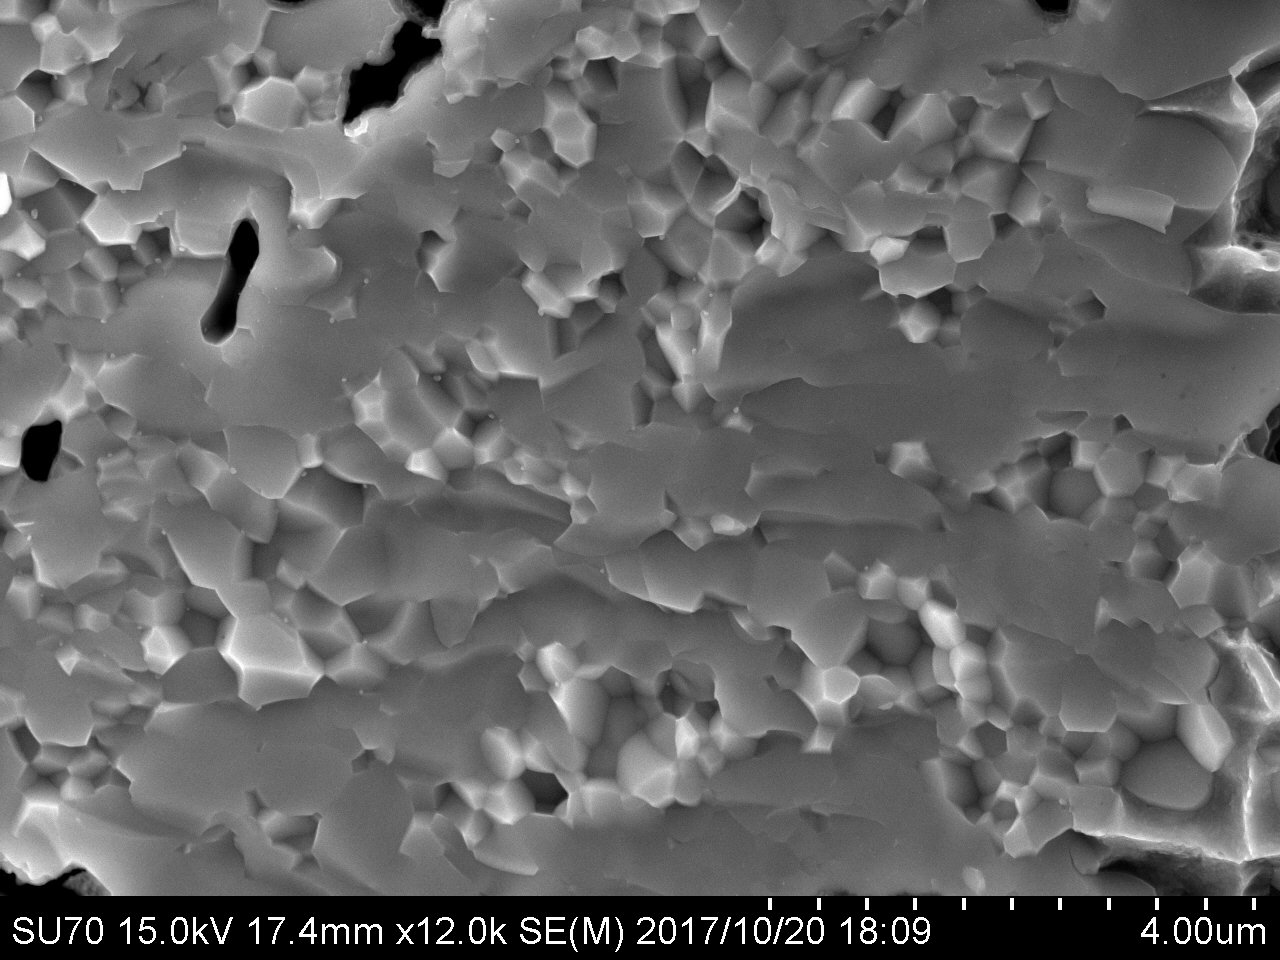
\includegraphics[width=0.7 \linewidth]{figs/15Zn-sem.jpg}
				\end{column}
				\begin{column}{0.5\linewidth}
					\centering
					Ge添加あり\\
					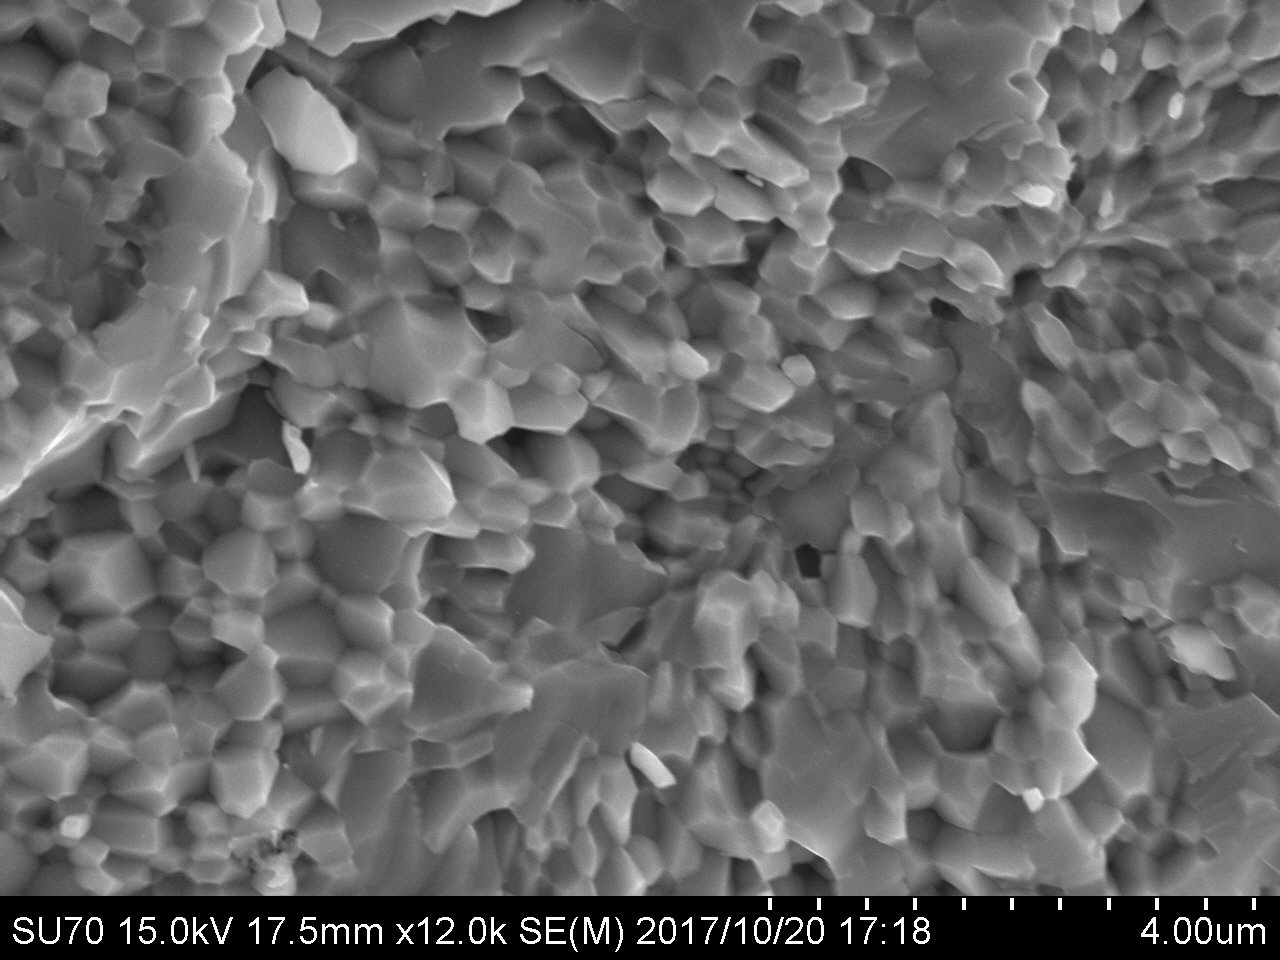
\includegraphics[width=0.7\linewidth]{figs/14Zn1Ge-sem.jpg}
				\end{column}
			\end{columns}
		\end{block}
		\begin{itemize}
			\item Ge添加なし:結晶の2次成長(粗大化)
			\item Ge添加:高温熱処理時に\textcolor{red}{結晶粒粗大化抑制効果}がある
		\end{itemize}
	\end{frame}

	\subsubsection{結晶粒径}
	\begin{frame}{結晶粒径}
		\begin{columns}
			\begin{column}{0.6\linewidth}
				\begin{itemize}
					\item 結晶粒界は主要なピンニング点であるため,\textcolor{red}{結晶粒は小さい方が良い}
					\item 全体的にGe無添加の方が結晶粒は小さい傾向になる.
					\item \textcolor{red}{Ge添加では高温熱処理において粗大化抑制}
				\end{itemize}
			\end{column}
			\begin{column}{0.4\linewidth}
				\centering
				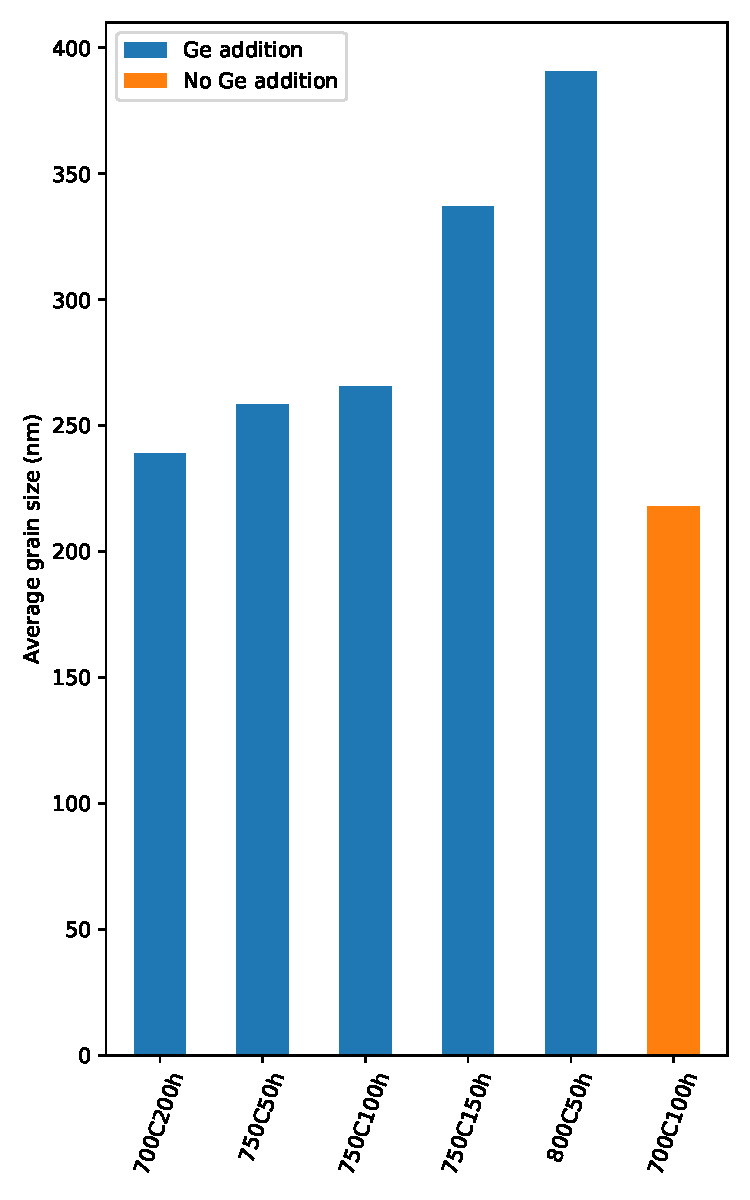
\includegraphics[width=0.9\linewidth]{figs/out.pdf}
			\end{column}
			
		\end{columns}
	\end{frame}

	\subsection{$J_\mathrm{c}$-$B$特性}
	\begin{frame}{$J_\mathrm{c}$-$B$特性}
		\begin{columns}
			\begin{column}{0.45\linewidth}
				\begin{itemize}
					\item Geの結晶粒粗大化抑制効果により,高温熱処理によって\textcolor{red}{化学量論性が完全・高磁界特性向上}かつ\textcolor{red}{低磁界側での比較的高い特性を維持}
				\end{itemize}
			\end{column}
			\begin{column}{0.55\linewidth}
				\centering
				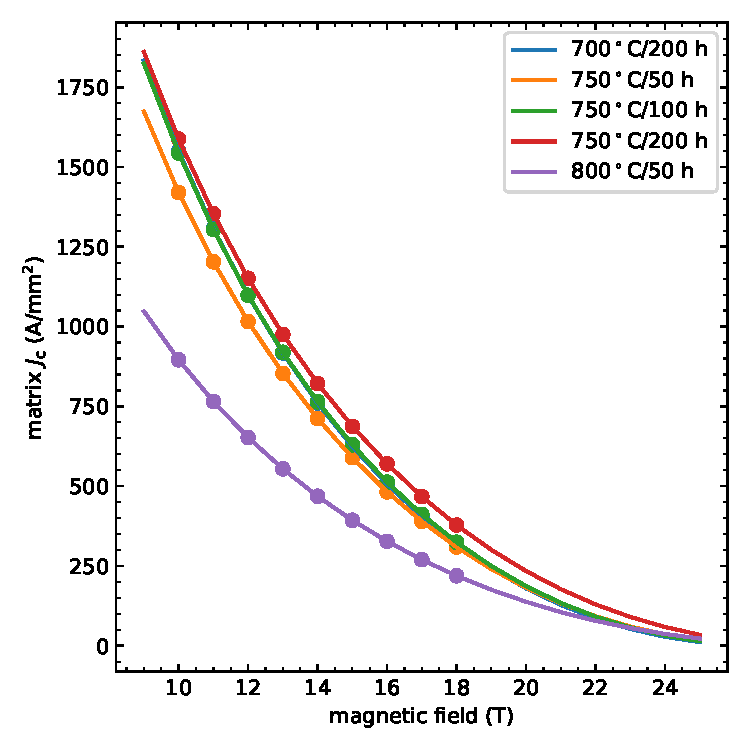
\includegraphics[width=0.9\linewidth]{figs/jcout.pdf}
				
			\end{column}
		\end{columns}

	\end{frame}

	\begin{frame}{$J_\mathrm{c}$-$B$特性:kramer plot}
		\begin{columns}
			\begin{column}{0.45\linewidth}
				\begin{itemize}
					\item 高温熱処理時に\textcolor{red}{結晶粒粗大化を抑制} \\
						→ \textcolor{red}{高磁界特性向上}
				\end{itemize}
			\end{column}
			\begin{column}{0.55\linewidth}
				\centering
				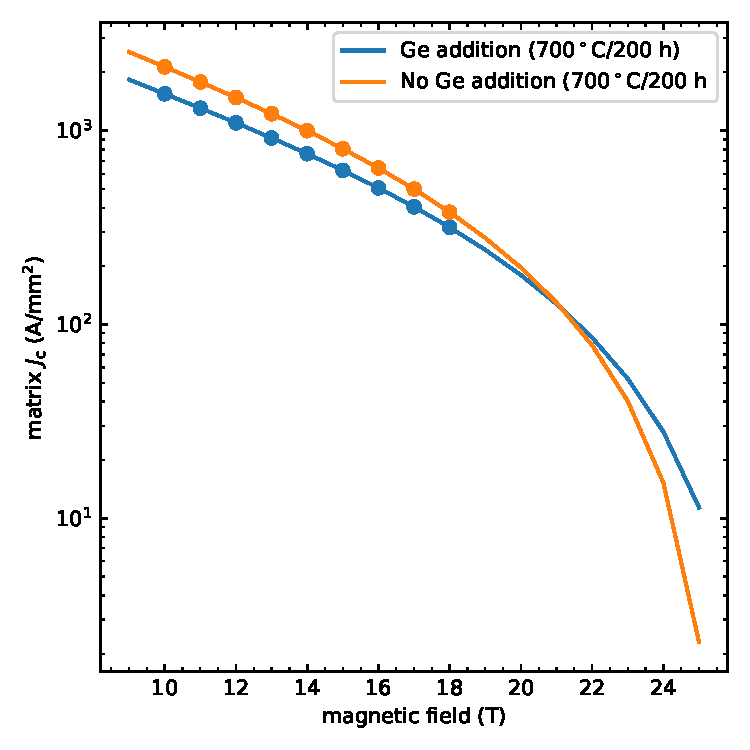
\includegraphics[width=0.9\linewidth]{figs/kramerout.pdf}
			\end{column}
		\end{columns}
	\end{frame}

	\begin{frame}{まとめ}
		\begin{itemize}
			\item 内部スズ法Nb\textsubscript{3}Sn線材に元素添加し,\textcolor{red}{微細組織制御}を行うことで\textcolor{red}{特性向上}を目指している.
			\item Cu母材へのZn, Ge同時添加を行った.ZnのNb\textsubscript{3}Sn生成促進効果と\textcolor{red}{Geの特異なNb\textsubscript{3}Sn周りGeリッチリング層によって結合電流の抑制効果を同時に得ようとした.}
			\item Ge添加によって結晶粒は僅かに粗大化するが,\textcolor{red}{高温熱処理時に結晶粒粗大化抑制効果}があることが明らかになった.
			\item 高温熱処理においても結晶粒がそれほど粗大化しないので\textcolor{red}{高磁場特性が向上した.}
		\end{itemize}
	\end{frame}

	\begin{frame}{今後の研究計画}
		\begin{itemize}
			\item Sn芯へのTi添加ではSn, Tiの分布が不均一であることが分かった.
			\item Sn, Ti分布の分布の均一性を解決することが課題
			\item 様々なTi添加方法を検討し,微細組織と$J_\mathrm{c}$特性を評価する
		\end{itemize}
		
	\end{frame}
	\begin{frame}{}
		\centering
		{\LARGE おわり}
	\end{frame}
\end{document}
